\section{Scheduling and execution}
\label{sec:app:scheduling_execution}
This section provides more details about tasks, task creation and scheduling (Section~\ref{sec:architecture}) as well as about our scheduler implementation~\ref{sec:implementation}.

\subsection{Task creation}
\label{sec:app:scheduling_execution_task_creation}

Tasks are created based on the blocks in a program.
Specifically, a block $B$ in the program is mapped to a set $T(B)$ of tasks.
Since a block may be executed multiple times, multiple instances of $T(B)$ can be created at runtime.

CL and CC blocks are mapped to CPS tasks only.
QL and QC blocks are mapped to a sequence of CPS- and QPS tasks.
\begin{itemize}
    \item CL block. A single \texttt{HostLocal} task is created.
    \item CC block. A single \texttt{HostEvent} task is created.
    \item QL block. If there is a single \texttt{run\_routine} call, a \texttt{LocalRoutine} task is created for the QPS, as well as a \texttt{PreCall} tasks and a \texttt{PostCall} task for the CPS.
    Two precedence constraints are added: the \texttt{PreCall} task precedes the \texttt{LocalRoutine} task, and the \texttt{LocalRoutine} task preceded the \texttt{PostCall} task.
    If there is a \texttt{join\_routines} on multiple local routine, multiple \texttt{PreCall}-\texttt{LocalRoutine}-\texttt{PostCall} task sets are created, without any dependencies between the task sets.
    \item QC block. If the request that is called from this block is for a single pair,
    a \texttt{SinglePair} task is created. If the request is for more than 1 pair, a \texttt{MultiPair} task is created. In both cases, an additional \texttt{PreCall} and a \texttt{PostCall} task are created with precedence constraints like for QL blocks.
    If there is a \texttt{join\_routines} on multiple request routines, multiple \texttt{PreCall}-Pair-\texttt{PostCall} task sets are created, without any dependencies between the task sets.
\end{itemize}
Figure~\ref{fig:app:task_creation} shows an overview of blocks and corresponding tasks and their precedence constraints.


\subsection{Predictable vs unpredictable programs}
Tasks are created based on the contents of a program instance, and their precedence relations are defined by the control-flow of the blocks in the program's host code.
Because of jump and branch instructions in the host code, a block may be executed zero, one or multiple times.
Furthermore, the exact number of executions of a block may not be known ahead of time.
For example, a program might loop through a sequence of blocks by using a conditional branch instruction at the end of the last block of the sequence.
The condition could depend on a runtime value (such as the result of a quantum measurement).
We say that control-flow is \textit{predictable} if it can be completely known before runtime. 
\textit{Unpredictable} control-flow, on the other hand, depends on values available only at runtime. 
For predictable programs, all its tasks can be created before runtime.
For unpredictable programs, (some of) its tasks must be created on-the-fly during program execution.
Figure~\ref{fig:app:linear_non_linear} illustrates the difference between predictable and unpredictable programs.

\begin{figure}[ht]
    \centering
    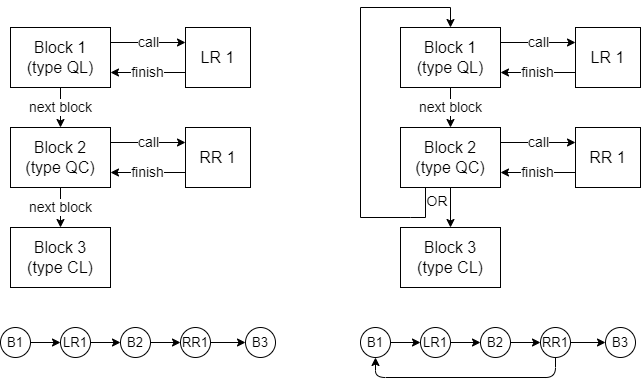
\includegraphics[width=\columnwidth]{figures/qoala/linear-non-linear.png}
    \caption{Schematic overview of the difference between predictable and non-predictable programs.
    The control-flow of the predictable program (left) is linear: first block 1 is executed (calling local routine (LR) 1), then block 2 (calling request routine (RR) 1), and finally block 3.
    Therefore, the number of tasks is fixed and known before execution.
    The non-predictable program is similar but after executing block 2, control-flow may go back to block 1 (again), depending on a runtime value (e.g. the result of RR 1).
    Hence, the number of times that blocks 1 and 2 are executed is not known beforehand, and therefore the number of tasks is also not known.
    }
    \label{fig:app:linear_non_linear}
\end{figure}

\begin{figure*}
    \centering
    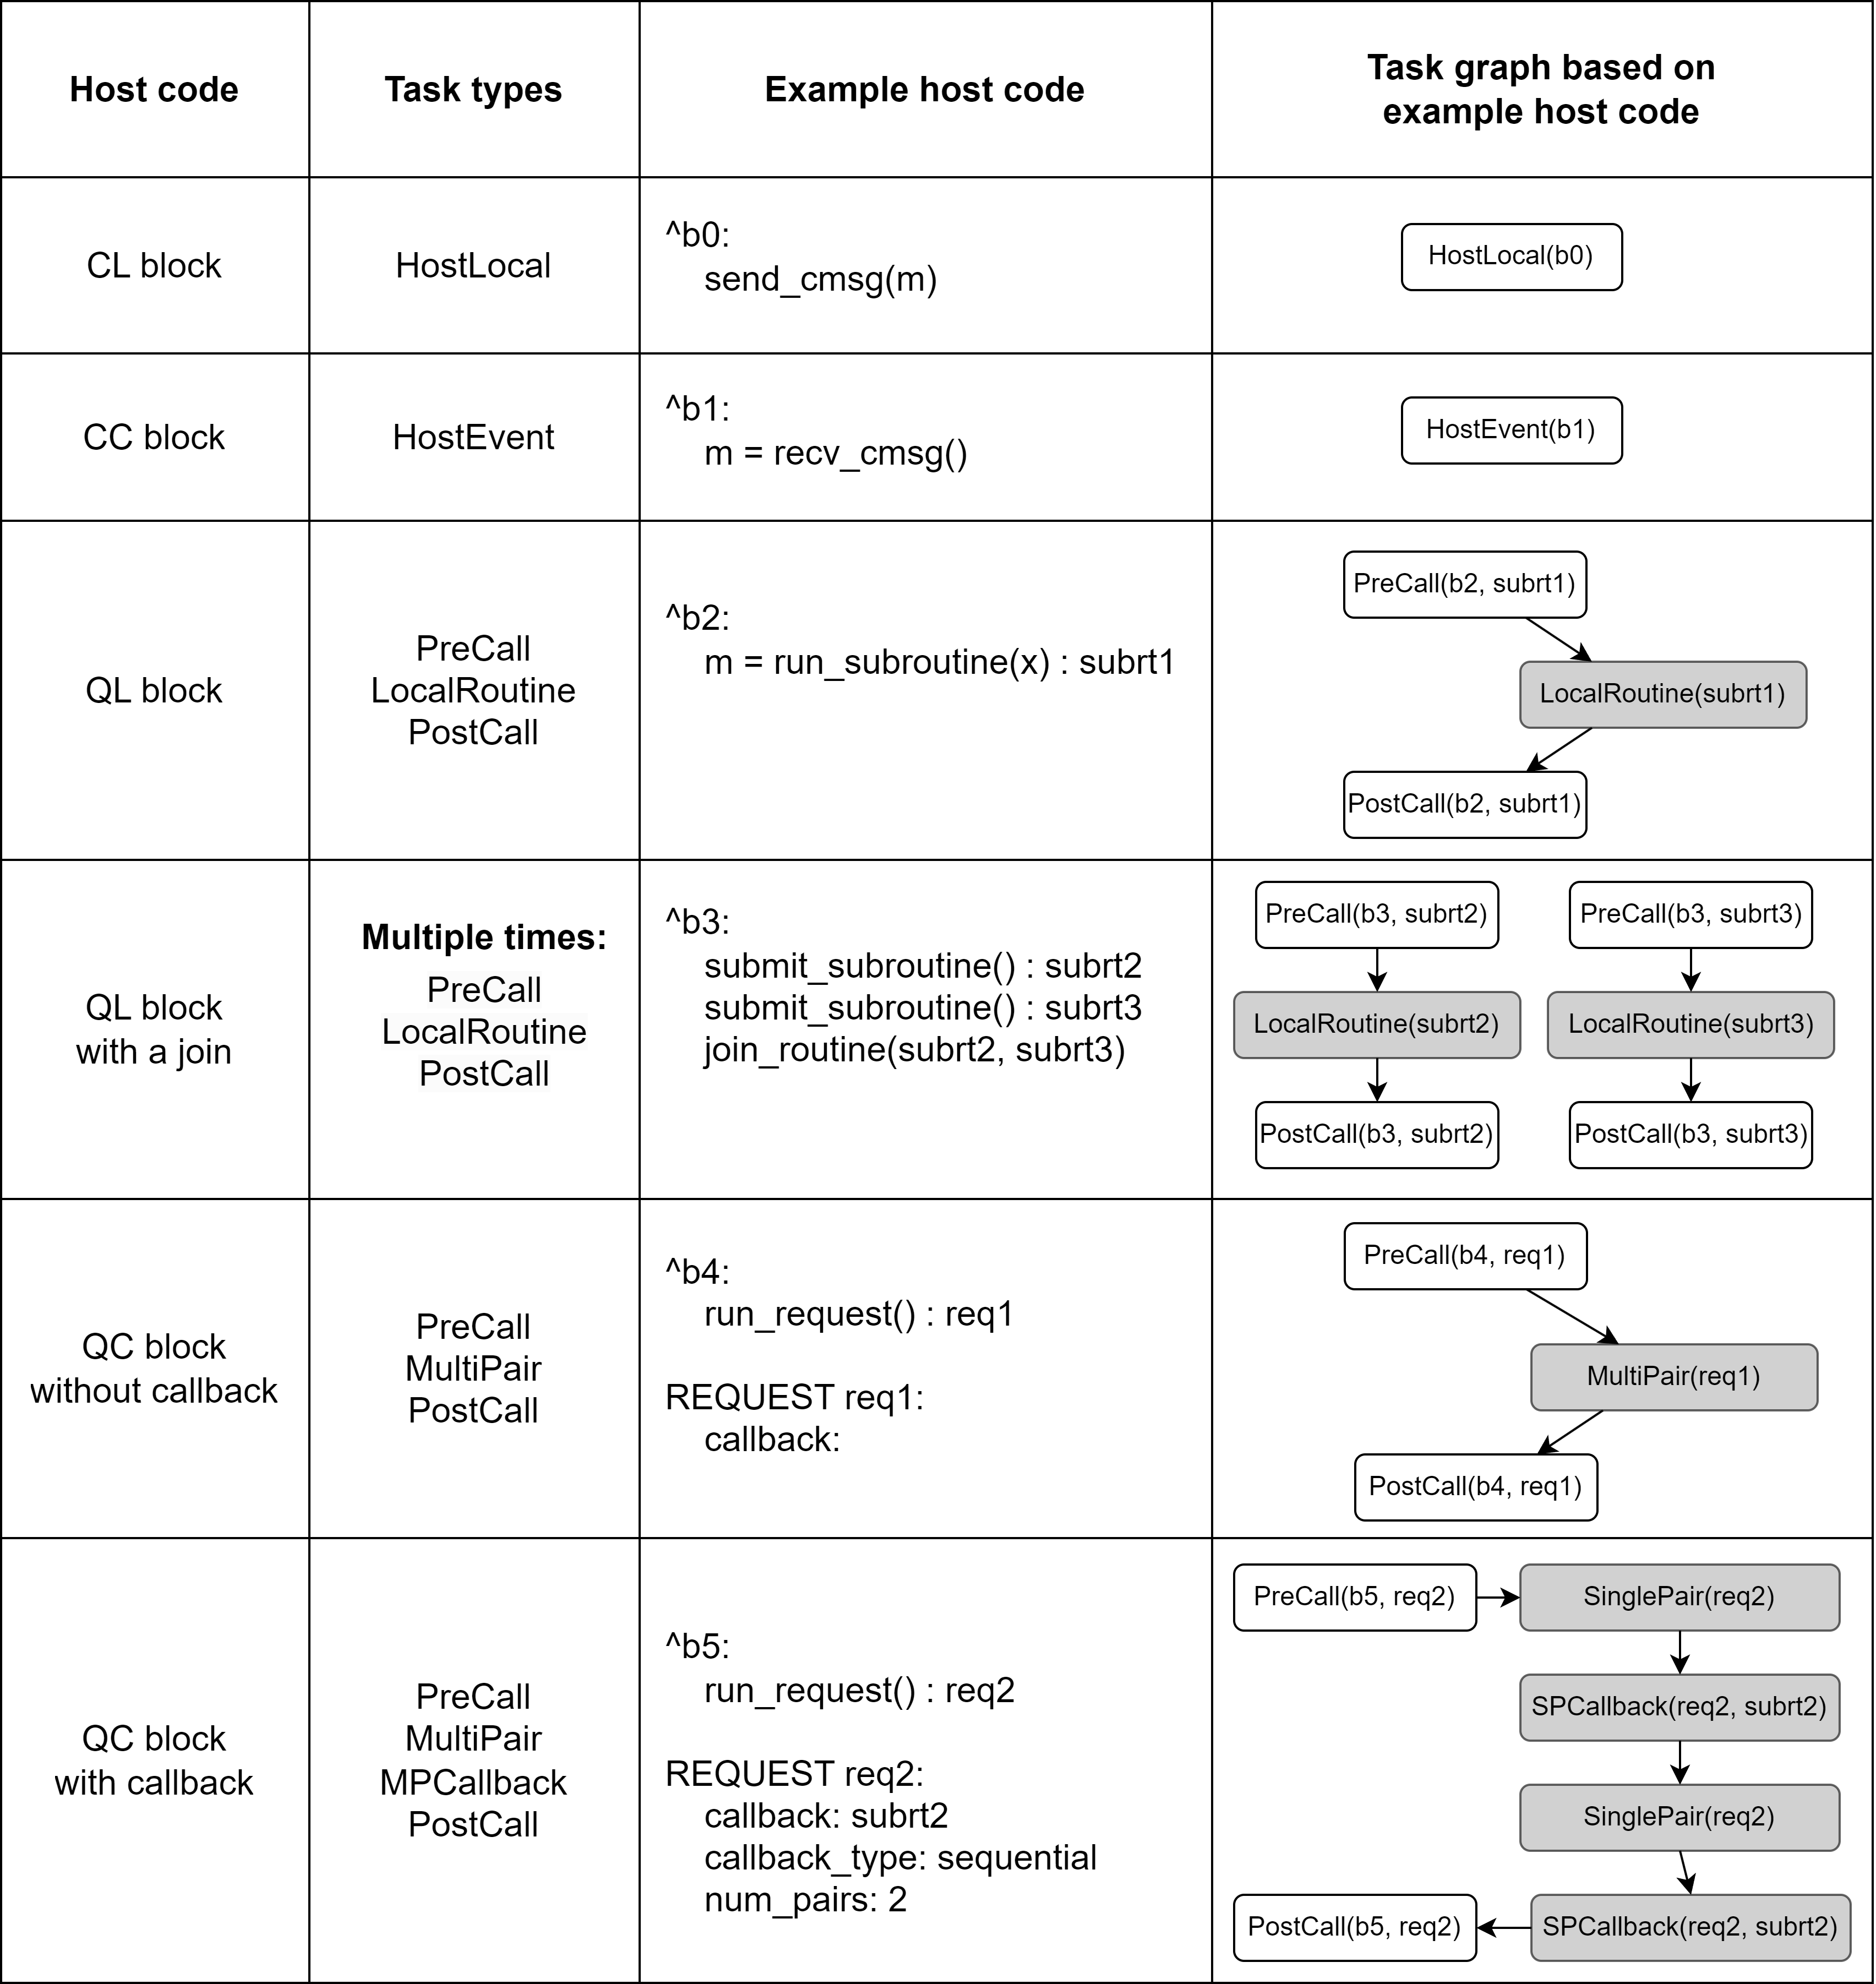
\includegraphics[width=\textwidth]{figures/qoala/task_creation.png}
    \caption{Overview of different host blocks with corresponding tasks. In the rightmost column, tasks with a dark background are QPS tasks, the others are CPS tasks. This example shows that tasks contain data about the program segment they correspond to, such as \texttt{LocalRoutine} tasks having the name of the routine they are executing.}
    \label{fig:app:task_creation}
\end{figure*}


\subsection{Task execution}
Tasks are executed by the CPS or the QPS, and the specific operations involved depend on the type of the task.

\textbf{\texttt{HostLocal} task execution.} A \texttt{HostLocal} task $t_{hl} = (P, B)$ for program instance $P$ and block $B$ is handled by executing each of the instructions in $B$. When the task finishes, the name of the next block to execute is recorded. If $B$ ends with a branch instruction, this is the target block; otherwise it is the next block in the program (if this was the last block, the next block is nil).

\textbf{\texttt{HostEvent} task execution}. A \texttt{HostEvent} task represents a block $B$ of type $CC$, which must start with exactly one \texttt{recv\_cmsg} instruction. Handling the task involves reading a message from the message buffer and assigning it to the result variable of the receive instruction. Then, the remaining instructions in $B$ are executed just like in a \texttt{HostLocal} task.


\textbf{\texttt{PreCall} task execution.} A \texttt{PreCall} task corresponds to a LR call instruction in Host code. The CPS allocates space in the shared memory for arguments and results. It then writes argument values to the shared memory.

\textbf{\texttt{PostCall} task execution.} A \texttt{PostCall} task corresponds to a LR call instruction in Host code. The CPS reads the results from the shared memory and copies them to the corresponding variables in the host local memory.

\textbf{\texttt{LocalRoutine} task execution.} A \texttt{LocalRoutine} task is executed by the QPS. It involves the following steps. First, based on information in the uses/keeps metadata, virtual quantum memory is allocated. Then all NetQASM instructions are executed, which may involve loading values from shared memory (reading arguments) and storing values to shared memory (populating results). Finally, quantum memory is freed.

\textbf{\texttt{SinglePair} task execution.} A \texttt{SinglePair} task is executed by the QPS. First, arguments are read from shared memory. Then, an EPR request (see Appendix~\ref{sec:app:entanglement_distribution}) is sent to the network controller.

\textbf{\texttt{MultiPair} task execution.} A \texttt{MultiPair} task is executed by the QPS. First, arguments are read from shared memory. Then, multiple EPR requests are sent to the network controller. Whether these requests are all sent at once or consecutively and waiting for intermediate responses is up to the implementer; the choice may depend on efficiency and resource considerations.

\textbf{\texttt{SinglePairCallback} and \texttt{MultiPairCallback} task execution.} First read results (from a \texttt{SinglePair} or \texttt{MultiPair} task) from shared memory. Then execute the callback routine just like a \texttt{LocalRoutine} task.

\subsection{Deadlines}
Deadlines can be specified for blocks relative to other blocks using the syntax:

\begin{lstlisting}[language=Pascal, caption=Pseudocode for the Algorithm, label=lst:pseudocode]
^block_0:
    ...

^block_1 { deadlines = [b0: 3ms] }:  // relative deadline of 3 ms compared to block_0
    ...
\end{lstlisting}

A relative deadline to some block $B$ is always with respect to the last task in $T(B)$, for the last task set instance (in case of multiple execution of this task set).
The deadline value may be an explicit value (like $3 ms$) or it can be in terms of EHI values, such as for example $0.1 * CC$ where $CC$ is the expected classical node-node latency provided by the EHI.

\subsection{Precedence constraints}
By default, blocks are executed in the order they are given in the program.
Blocks ending with a jump or branch instruction define precedence constraints at runtime for unpredictable programs.

Scheduling happens at runtime and involves choosing which task to execute next.
In Qoala, there are three schedulers per node: the \textit{CPS scheduler} controls task execution on the CPS,
the \textit{QPS scheduler} controls task execution on the QPS, and the \textit{node scheduler} controls the CPS- and QPS schedulers.
The CPS- and QPS schedulers are both processor schedulers.

\subsection{Scheduling overview}
In this and the following sections we describe the scheduler from our implementation (Section~\ref{sec:implementation}).

Each scheduler maintains their own task graph,
which is a directed acyclic graph (DAG) in which the nodes represent tasks and edges represent precedence constraints.
The node scheduler task graph contains all tasks (CPS or QPS) that are to be executed.
Each processor scheduler task graph is a partial copy of the node scheduler task graph containing only the tasks that can be executed by its own processor.
Edges in the node scheduler graph between heterogenous tasks (i.e. between CPS and QPS tasks) are represented in the partial processor graphs by the \textit{external dependencies} node attribute. See Figure~\ref{fig:app:task_graph_partial} for an example.
When a processor scheduler finishes a task, it is removed from the task graph and a signal is sent to the node scheduler.
The node scheduler updates its own task graph accordingly, and may then add new tasks to the task graph of the processor scheduler.
Note that although the processor task graphs are accessible by both the owning processor scheduler and the node scheduler, there are no read/write conflicts
since tasks can only be added by the node scheduler, and tasks can only be removed by the processor scheduler.

\subsection{Task graph}
A task graph consists of 
\begin{itemize}
\item \textit{tasks} to be scheduled (the nodes),
\item \textit{precedence constraints} between the tasks (precedence edges),
\item \textit{external precedence constraints} for tasks in the case of processor task graphs (annotated on the nodes),
\item \textit{relative deadlines} between tasks (deadline edges),
\item \textit{trigger annotations} for some tasks (like incoming messages or network schedule timestamps)
\end{itemize}


Upon program instantiation, all created tasks are added to the node scheduler task graph, and the relevant tasks are added to the processor schedulers.
The number of tasks that are created (and can hence be added to the task graphs) depends on the predictability of the program.
During runtime, the node scheduler may create new tasks based on the control-flow of the program.

\begin{figure}[ht]
    \centering
    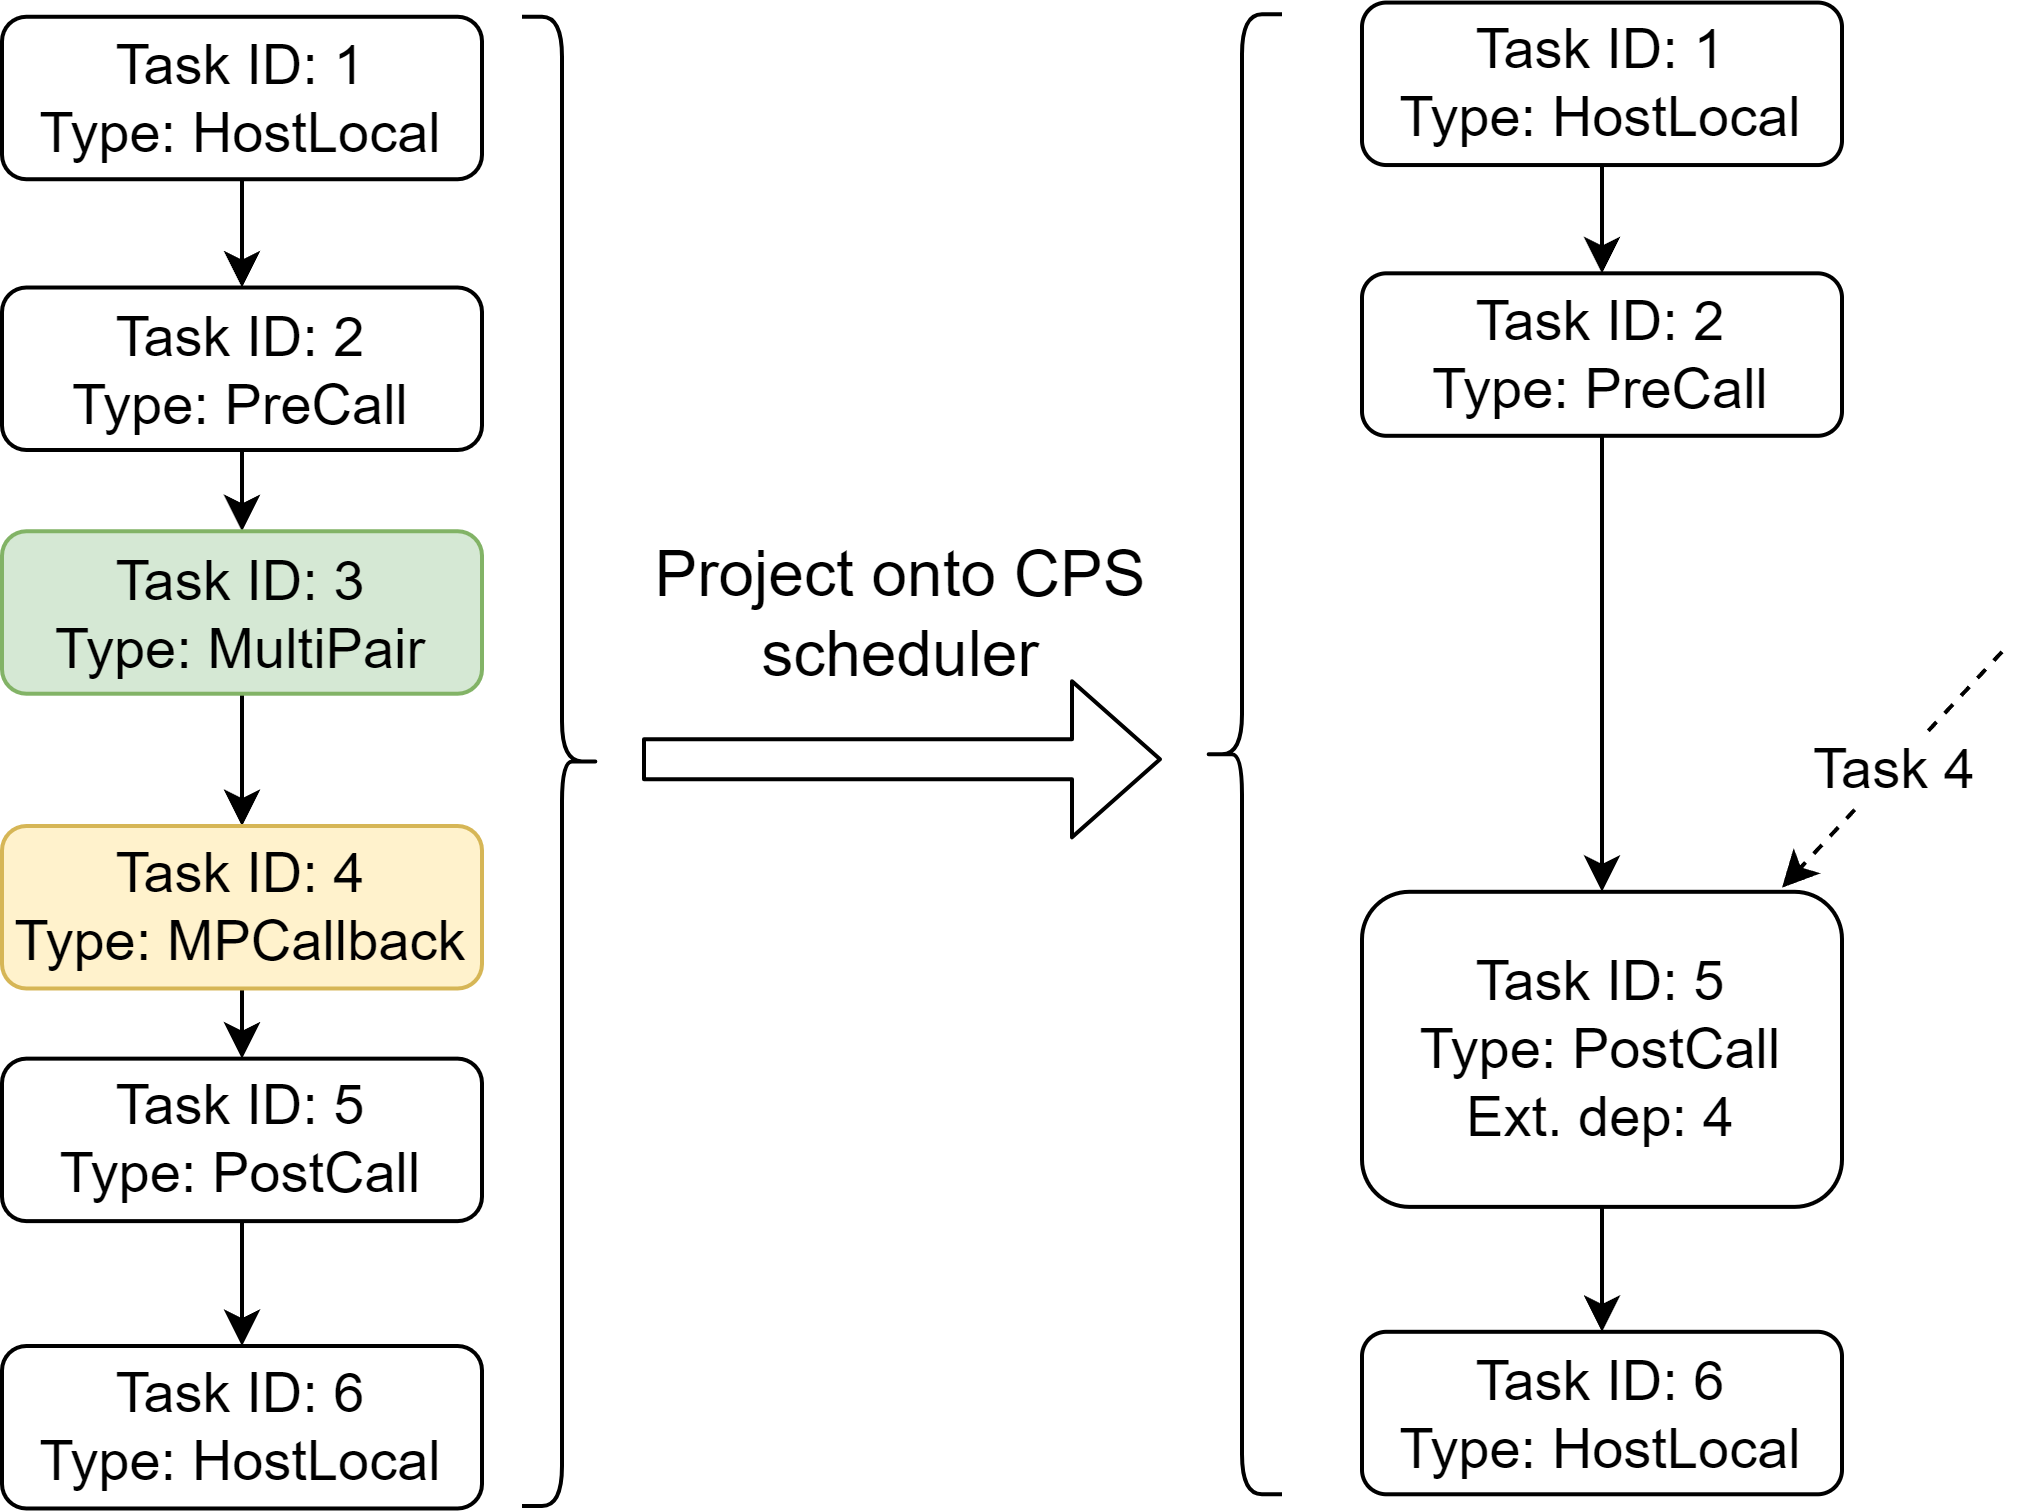
\includegraphics[width=\columnwidth]{figures/qoala/task_graph_partial.png}
    \caption{
        Example of a mapping from a full task graph (containing both CPS and QPS tasks) to a partial graph (containing only CPS tasks).
        Task 5 depends on task 4, which is external from the perspective of the CPS scheduler (indicated using the \texttt{external-dependencies} attribute).
        Note that Task 3 is not needed at all in the partial graph; only the dependency on task 4.
    }
    \label{fig:app:task_graph_partial}
\end{figure}

\subsection{Task graph splitting}
\label{sec:app:task_graph_splitting}
The node scheduler creates a heterogenous task graph consisting of both CPS and QPS tasks.
This graph needs to be split into a partial CPS and a partial QPS graph.
This is done using the following algorithm.

We consider creating the partial graph for the CPS, and hence the QPS is `the other processor'.
For the partial graph of the QPS the procedure is exactly the same but with reversed roles.

For a heterogenous task graph $G$ containing tasks $T$ (all tasks for both CPS and QPS), precedence constraints $P$ ($(t_1, t_2) \in P$ means that $t_1$ must precede $t_2$), compute the partial CPS graph $G_{CPS}$ as follows:

\begin{itemize}
    \item Split $T$ into a set $T_{CPS}$ consisting of all tasks that run on the CPS, and $T_{QPS}$ consisting of all other tasks in $T$. $G_{CPS}$ will consist of only tasks in $T_{CPS}$.
    \item Let $P_{CPS} \subset P$ consist of all precedence constraints $(t_1, t_2)$ where $t_1 \in T_{CPS}$ and $t_2 \in T_{CPS}$.
    These constraints will remain the same in $G_{CPS}$ since they are between tasks in $T'$.
    \item Compute the `immediate cross-predecessors' set $I$ of all tasks $t_{cp} \in T_{QPS}$ such that there exists a task $t \in T_{CPS}$ and $(t_{cp}, t) \in P$.
    In other words, $I$ contains all tasks running on the QPS that are immediate predecessors of CPS tasks.
    \item For each $t_i \in I$, compute the `closest CPS ancestor' task $t_{anc} \in T_{CPS}$, which is a CPS task that has a direct precedence constrain with the closest ancestor of $t_i$.
    Add $(t_{anc}, t_i)$ to the precedence constraints of $G_{CPS}$.
\end{itemize}

\subsection{Scheduler communication}
Here we describe how the schedulers communicate in our implementation (Section~\ref{sec:implementation}).

The three schedulers need to exchange information in order to work together.
All schedulers can broadcast a \textit{signal} with short information such as `task N completed' or `memory freed'. Each scheduler receives these signals.
Furthermore, the following read and write access is given:
\begin{itemize}
    \item The CPS scheduler can read from the completed task ID list of the QPS and vice versa. This makes it possible for the CPS (QPS) scheduler to directly update their remote dependencies without having to wait for a signal from the node scheduler, leading to overall improvement in efficiency
    \item The node scheduler can add new tasks to the partial graphs of the CPS and QPS. Note that the node scheduler will only add tasks to the partial graph of a processor scheduler when this scheduler is in a waiting state; that is, after the processor scheduler has sent a `waiting` signal and before the node scheduler has sent a `task added` signal (only after this signal will the processor scheduler) continue. In this way, there are no read/write conflicts in the partial graphs of processor schedulers.
    \item The CPS (QPS) scheduler can only remove tasks from its own partial graph, not add any.
\end{itemize}

\begin{figure*}[ht]
    \centering
    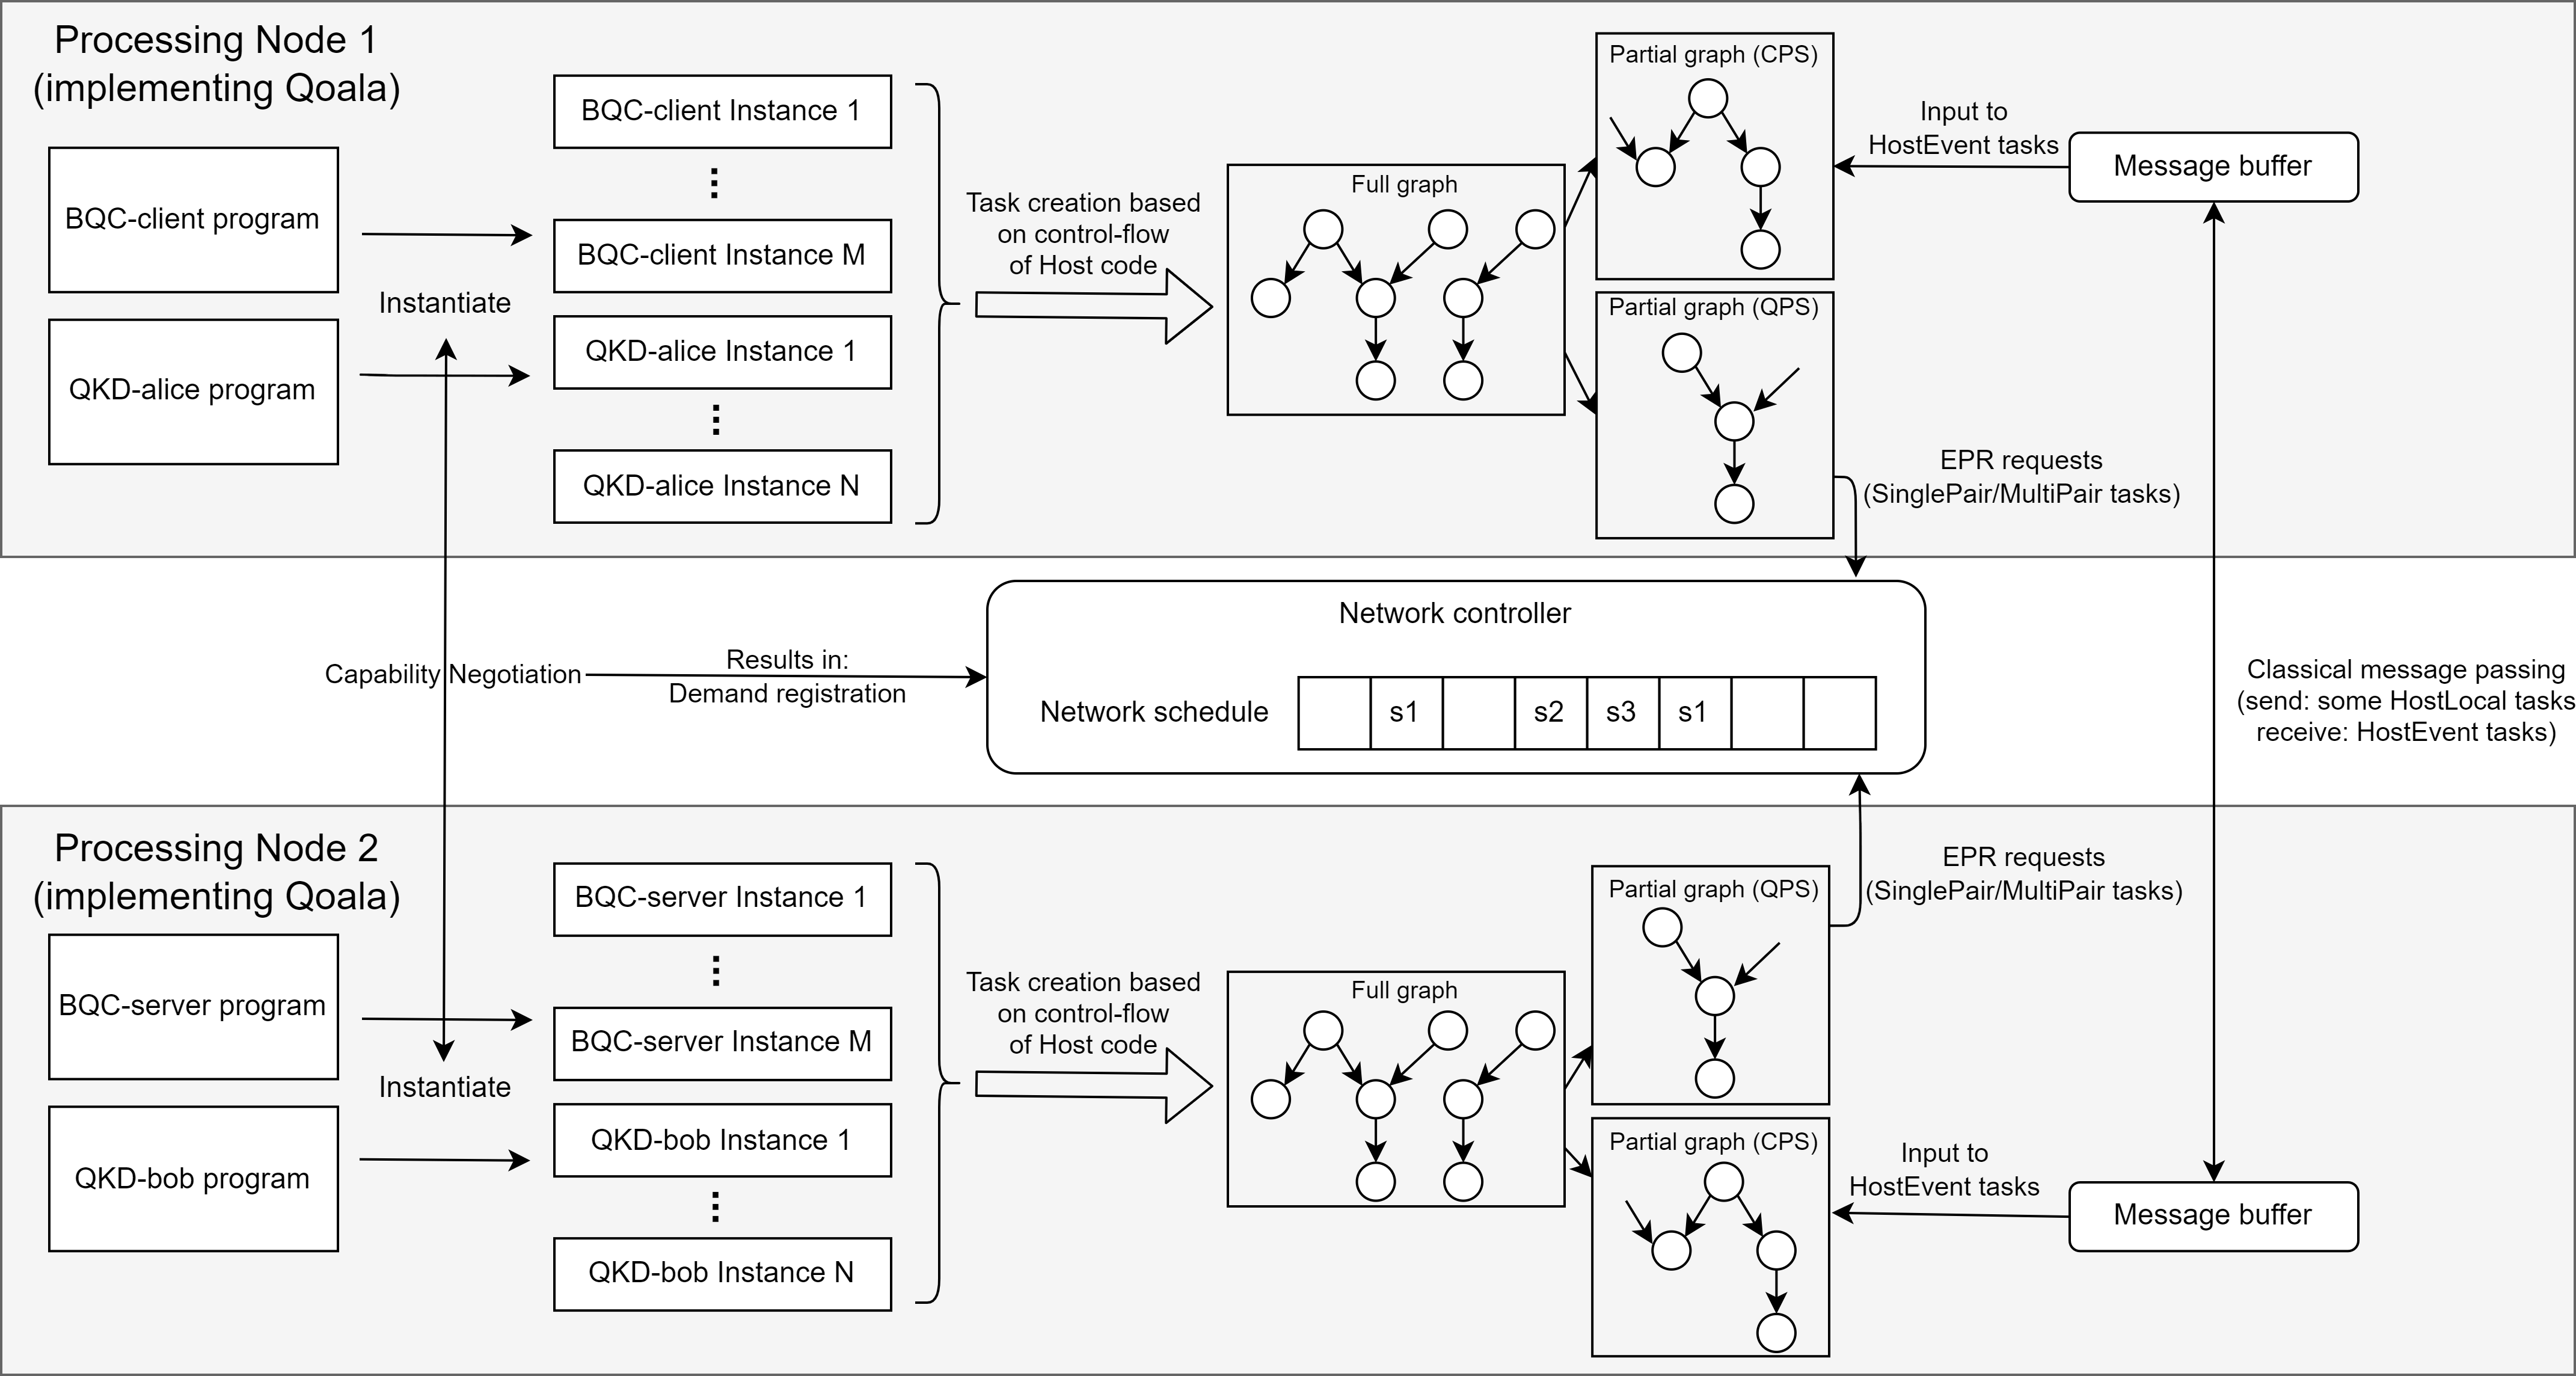
\includegraphics[width=\textwidth]{figures/qoala/runtime_detailed.png}
    \caption{Detailed runtime overview}
    \label{fig:app:runtime_detailed}
\end{figure*}


\subsection{Node scheduler algorithm}
Below we describe the high-level steps involved in the node scheduler algorithm implementation of Section~\ref{sec:implementation}.
\label{sec:app:node_scheduler_algorithm}
\begin{enumerate}
    \item Split the current task graph into a partial CPS graph and a partial QPS graph. For the algorithm, see Appendix~\ref{sec:app:task_graph_splitting}.
    \item Add the CPS (QPS) tasks to the partial graph of the CPS (QPS) scheduler
    \item Wait for a `task finished` signal from either CPS or QPS scheduler
    \item Remove the corresponding task from the task graph.
    \item If the finished task was a \texttt{HostLocal} task for some program instance P, and if the CPS partial graph is empty, check which block the program instance should jump to. This information is given by the task itself (and stored in the completed task list of the CPS scheduler), after evaluating the last instruction (a jump or branch instruction) in the BB that the task represented. For this new BB, create corresponding tasks for both the CPS and QPS. Task creation is discussed in Appendix~\ref{sec:app:scheduling_execution_task_creation}.
    \item If the task graph is empty, idle until new programs are instantiated.
    \item Go back to step 1.
\end{enumerate}

Note that the role of the node scheduler is much smaller when only predictable programs are run.
When predictable programs are instantiated, all of their tasks are created at once, resulting in a large task graph in the node scheduler, which never gets new tasks created at runtime.
In this scenario, after steps 1 and 2 the CPS and QPS schedulers possess a partial graph which will never get any new tasks.
Both processor schedulers will work on their tasks until they are both empty, after which all program instances have finished. Meanwhile, the node scheduler just loops through steps 1, 2, 3 and 6, not doing anything.

\subsection{CPS scheduler algorithm}
Below we describe the high-level steps involved in the CPS scheduler algorithm implementation of Section~\ref{sec:implementation}.
\begin{enumerate}
    \item Check which new tasks were completed by the QPS by reading from the shared task memory. Remove external dependency edges that correspond to QPS tasks that have completed.
    \item Find all tasks in the partial graph that are ready to execute. These are tasks that fulfill all following requirements:
        \begin{itemize}
            \item The task has no incoming precedence constraints (there are no unfinished tasks in the task graph that must precede this task)
            \item The task has no external precedence constraints (there are no unfinished QPS tasks that must precede this task)
            \item If the task is a \texttt{HostEvent} task, there must be at least one message in the CPS' message buffer
            \item If the task has a specific start time, the current time should be at least the start time
        \end{itemize}
    \item If there is no task ready to execute, send a `waiting` signal and wait until a signal is received that indicates one of the following events:
        \begin{itemize}
            \item The node scheduler has added one or more tasks to the partial graph
            \item The QPS scheduler has completed a task
            \item The start time has arrived of one of the tasks that were previously not ready only because their start time had not yet passed
            \item One or more new messages have been put into the message buffer
        \end{itemize}
        After one of these signals is received, go back to step 1.
    \item If there is at least one task ready to execute, choose which one to execute now. This depends on the scheduling policy that is being used. The policy may or may not use information about the deadlines of the available tasks. Scheduling policies that were implemented for our evaluation are described in Appendix~\ref{sec:app:evaluation}.
    \item If the task failed, go back to step 1
    \item If the task completed, remove it from the partial graph, add its ID to the completed task ID list, and broadcast a signal that the task was finished. If the task was a \texttt{HostLocal} task, then also store (in the completed task list) an entry containing the name of the next block to execute. (In this way, the node scheduler knows which task(s) to create and add to the full task graph. See Appendix~\ref{sec:app:scheduling_execution_task_creation} for more details.)
    Update the deadlines of all other tasks in the task graph.
    Then go back to step 1.
\end{enumerate}

\subsection{QPS scheduler algorithm}
Below we describe the high-level steps involved in the QPS scheduler algorithm implementation of Section~\ref{sec:implementation}.
\begin{enumerate}
    \item Check which new tasks were completed by the CPS by reading from the shared task memory. Remove external dependency edges that correspond to CPS tasks that have completed.
    \item Find all tasks in the partial graph that are ready to execute. These are tasks that fulfill all following requirements:
        \begin{itemize}
            \item The task has no incoming precedence constraints (there are no unfinished tasks in the task graph that must precede this task)
            \item The task has no external precedence constraints (there are no unfinished CPS tasks that must precede this task)
            \item If the task is a \texttt{SinglePair} or \texttt{MultiPair} task, the current time should be the beginning of a network time slot that corresponds to this task. (For example, if the task is for creating EPR pairs for program instance 1 on this node (called `Alice') and program instance 2 on node `Bob', then the current time should be the start of a $(Alice, 1, Bob, 2)$ time slot).
            \item If the task has a specific start time, the current time should be at least the start time
        \end{itemize}
    \item If there is no task ready to execute, wait for a signal that indicates one of the following events:
        \begin{itemize}
            \item The node scheduler has added one or more tasks to the partial graph
            \item The CPS scheduler has completed a task
            \item The start time has arrived of one of the tasks that were previously not ready only because their start time had not yet passed
            \item The start of a time slot has arrived which corresponds to one of the tasks that were previously only blocked on the arrival of this time slot
        \end{itemize}
        After one of these signals is received, go back to step 1.
    \item If there is at least one task ready to execute, choose which one to execute now. This depends on the scheduling policy that is being used. The policy may or may not use information about the deadlines of the available tasks.
    \item If the task failed, go back to step 1
    \item If the task completed, remove it from the partial graph, add its ID to the completed task ID list, and broadcast a signal that the task was finished.
    Update the deadlines of all other tasks in the task graph.
    Then go back to step 1.
\end{enumerate}


\subsection{Task graph updates}
The node scheduler may add tasks to the current task graph of the CPS or QPS.
When a processor scheduler has finished a task, it is removed from the task graph.
This has the following effects:
\begin{itemize}
    \item Precedence edges from this task are removed, potentially making other tasks available for execution
    \item The time of finishing is recorded; and the deadlines and relative deadlines of all other tasks are updated accordingly
\end{itemize}



\subsection{Linear graphs}

When instantiating a program multiple times (for example instantiating a BQC program 1000 times), one has the option to linearize the graphs. Each instantiation has its own graph,
and the full graph of all instances result in many independent tasks.
One can force all instances to be run in sequence, rather than interleaved, resulting in a linear chain of single-instance graphs. This is done using the following algorithm:

\begin{itemize}
    \item For each pair $(i_1, i_2)$ of consecutive instances, add a precedences constraint between the last tasks(s) of $i_1$ and the first task(s) $i_2$.
\end{itemize}

\begin{figure*}
    \newcommand{\networkcontrollerfigheight}{4.5cm}
    \centering
    \subfloat[\centering \label{fig:app:network_controller_requests}]{{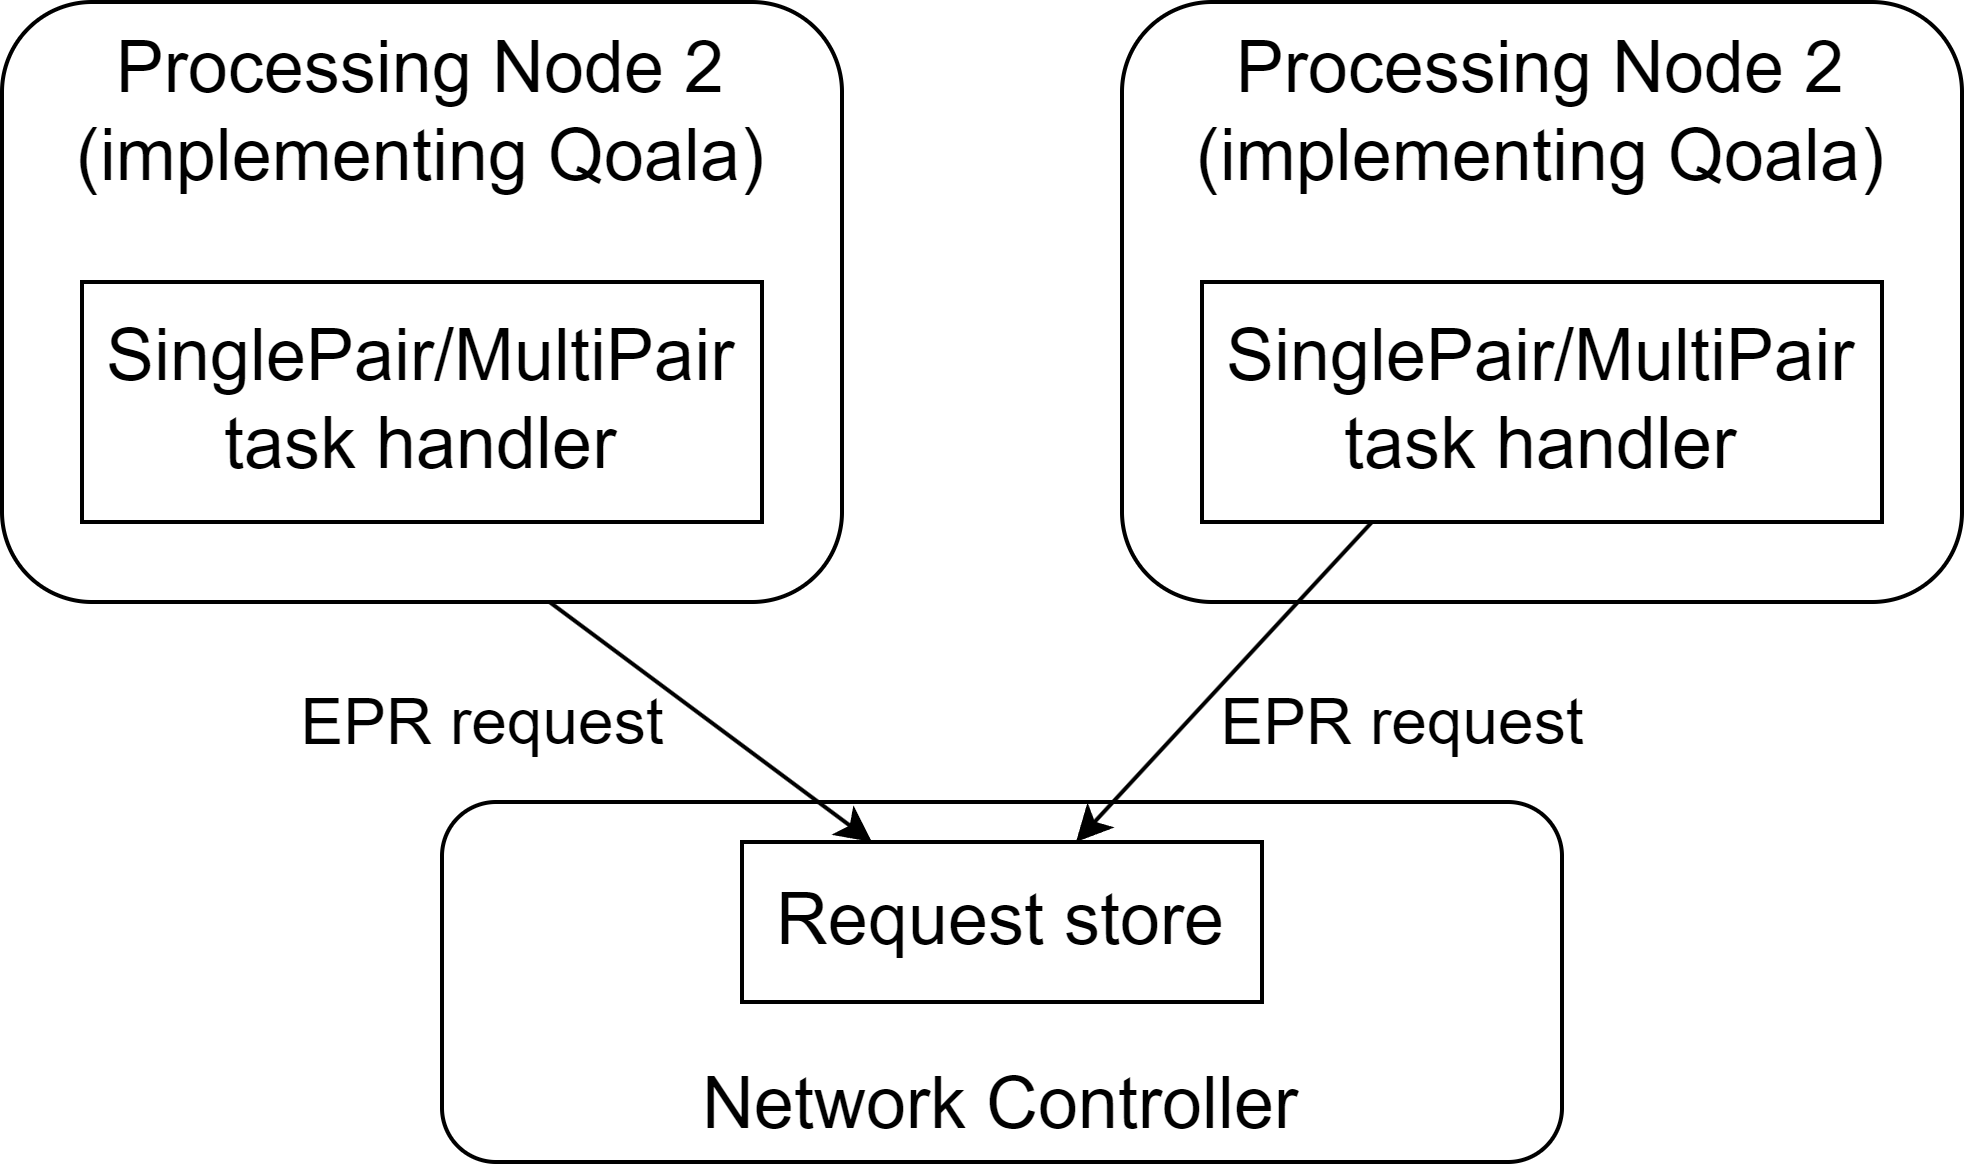
\includegraphics[height=\networkcontrollerfigheight, keepaspectratio]{figures/qoala/network_controller_requests.png}}}%
    \qquad
    \subfloat[\centering \label{fig:app:network_controller_requests_distributed}]{{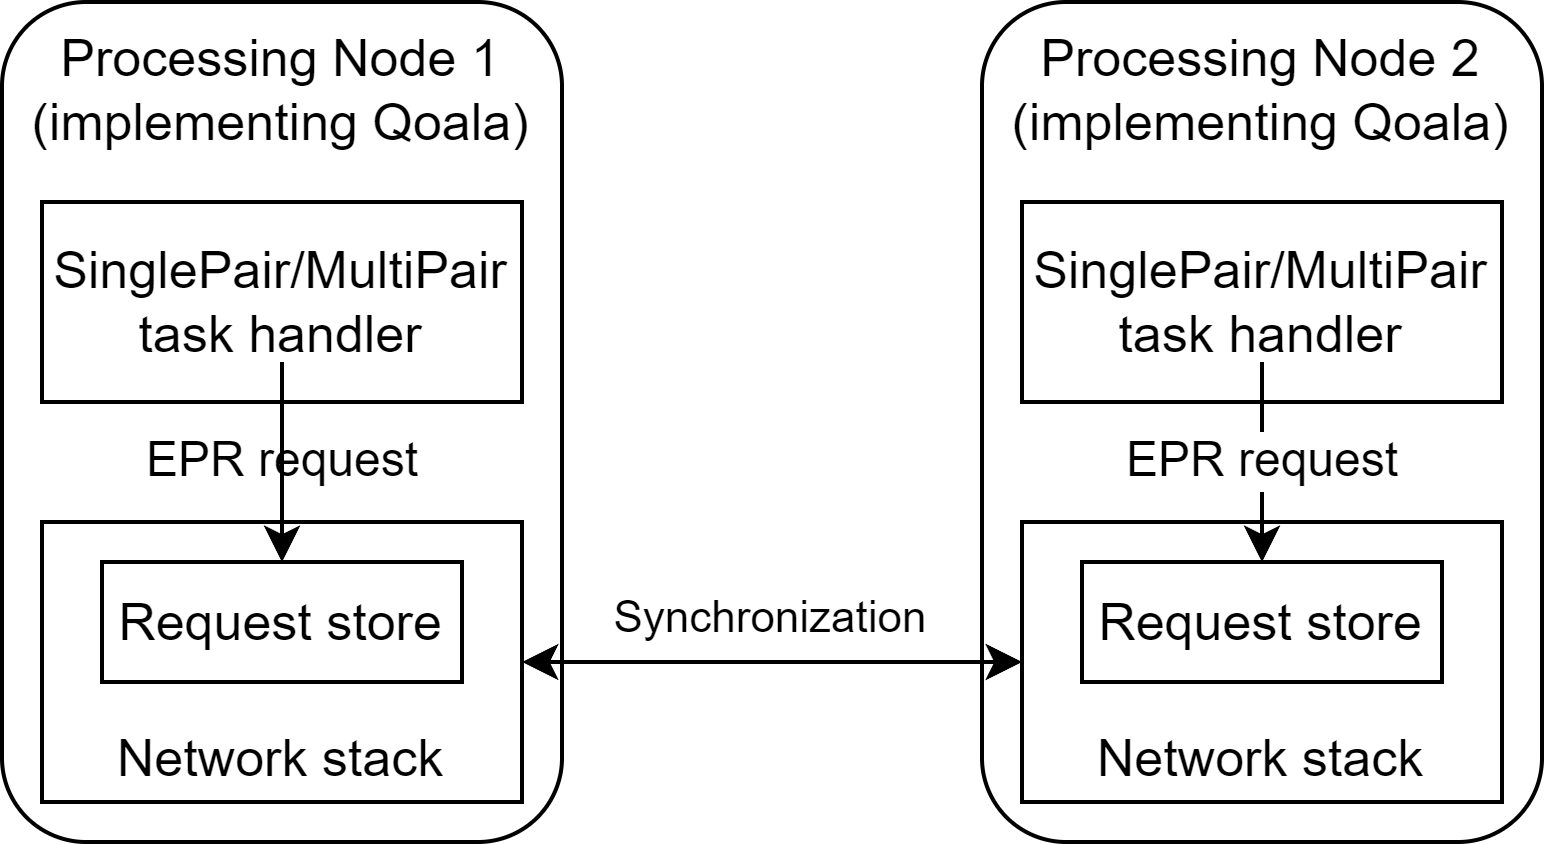
\includegraphics[height=\networkcontrollerfigheight, keepaspectratio]{figures/qoala/network_controller_requests_distributed.png}}}%
    \caption{
    Different implementations of network controller and network stack.
    (a) The network controller is centralized and the nodes send requests to this controller
    whenever they are executing \texttt{SinglePair} or \texttt{MultiPair} tasks.
    (b) The network controller is distributed over the nodes. Inside each node there is a network stack which autonomously talks with the network stack of other nodes and synchronizes entanglement generation.
    Execution of \texttt{SinglePair} and \texttt{MultiPair} tasks involves sending a request to the network stack within the node, which then handles pair generation by synchronizing with the network stack in other nodes.
    }%
    \label{fig:app:network_controller_types}
\end{figure*}


\subsection{Estimating task durations}
The scheduler uses the EHI to estimate the duration of a task.
This duration may then be used by the scheduler to decide which task to execute when.
In our implementation, the scheduler does not make use of these estimates, but we did implement a simple estimator algorithm:

The estimated duration $E$ of a task is computed as follows:
\begin{itemize}
    \item For a \texttt{HostLocal} or \texttt{HostEvent} task representing a program block $B$, $E$ is $N \cdot$ \texttt{host\_latency} where $N$ is the number of HostLanguage operations in $B$ and \texttt{host\_latency} is given in the EHI.
    \item For a \texttt{LocalRoutine} tasks representing a block that call a NetQASM routine $S$, 
        $E$ is the sum of estimated durations of each NetQAM instruction in $S$. The duration of each quantum instruction is obtained from the EHI, and the duration of each classical instruction is given by the \texttt{qnos\_latency} entry in the EHI.
    \item For a \texttt{SinglePair} or \texttt{MultiPair} task based on a block that calls a request $R$ for $N$ EPR pairs, $E$ is $N$ times the duration of a single EPR generation as listed in the EHI.
    \item For \texttt{PreCall} and \texttt{PostCall} tasks, the duration is set to the \texttt{host\_latency} entry in the EHI.
\end{itemize}

\subsection{Batches}
A program may be submitted for execution in a batch.

A batch $B$ consists of a program $P$, the number of execution $N$ and inputs for each execution. Based on this, $N$ program instances are created.


\subsection{Memory allocation}
Consider the following scenario: at runtime, all but one physical qubits of the processing node are in use (holding a state which is acted upon by tasks that still need to run).
The scheduler sees that two QPS tasks, coming from two different programs) are available to be run at this moment and has to make a choice.
Task A uses virtual qubit 0, and task B uses virtual qubit 1 and 2. 



\subsection{Entanglement Distribution}
\label{sec:app:entanglement_distribution}
Qoala only defines how program are executed on a node in a quantum network,
and not how and when entanglement is created between nodes.
However, Qoala does assume certain things about how nodes can interact with the entanglement distribution system, however this is implemented.
The assumption about entanglement generation are as follows.

\textbf{Network controller with time slots.}
Conceptually, there is a network controller that oversees entanglement generation and distribution across the whole network.
Qoala does not care whether this controller is implemented as a single entity, or is distributed in some way across multiple (processing) nodes (Figure~\ref{fig:app:network_controller_types}).
The network controller maintains a global timeline divided into \textit{time slots}, which can have arbitrary length.
Each time slot may be assigned to a \textit{session}, which is a 4-tuple $(N1, P1, N2, P2)$ where $N1$ ($N2$) is the name of a node in the network and $P1$ ($P2$) is an ID of a program instance running within $N1$ ($N2$).
A session hence represents a pair of running program instances across two nodes, and it is such pairs of program instances that want to create entanglement with each other. 
If a time slot is assigned to some session $(N1, P1, N2, P2)$, only program instances $P1$ and $P2$ (on nodes $N1$ and $N2$) may create entanglement with each other during this time slot.

Populating the network controller's time slot with sessions is the result of (1) demand registration by nodes in the network, followed by (2) network schedule generation by the network controller itself, which we do not consider here (Figure~\ref{fig:app:network_controller_setup}).
In the following, we simply assume that the network controller has a list of time slots assigned to sessions relating to program instances that are being run, and that these time slots are also known by the individual processing nodes.

\begin{figure*}[ht]
    \centering
    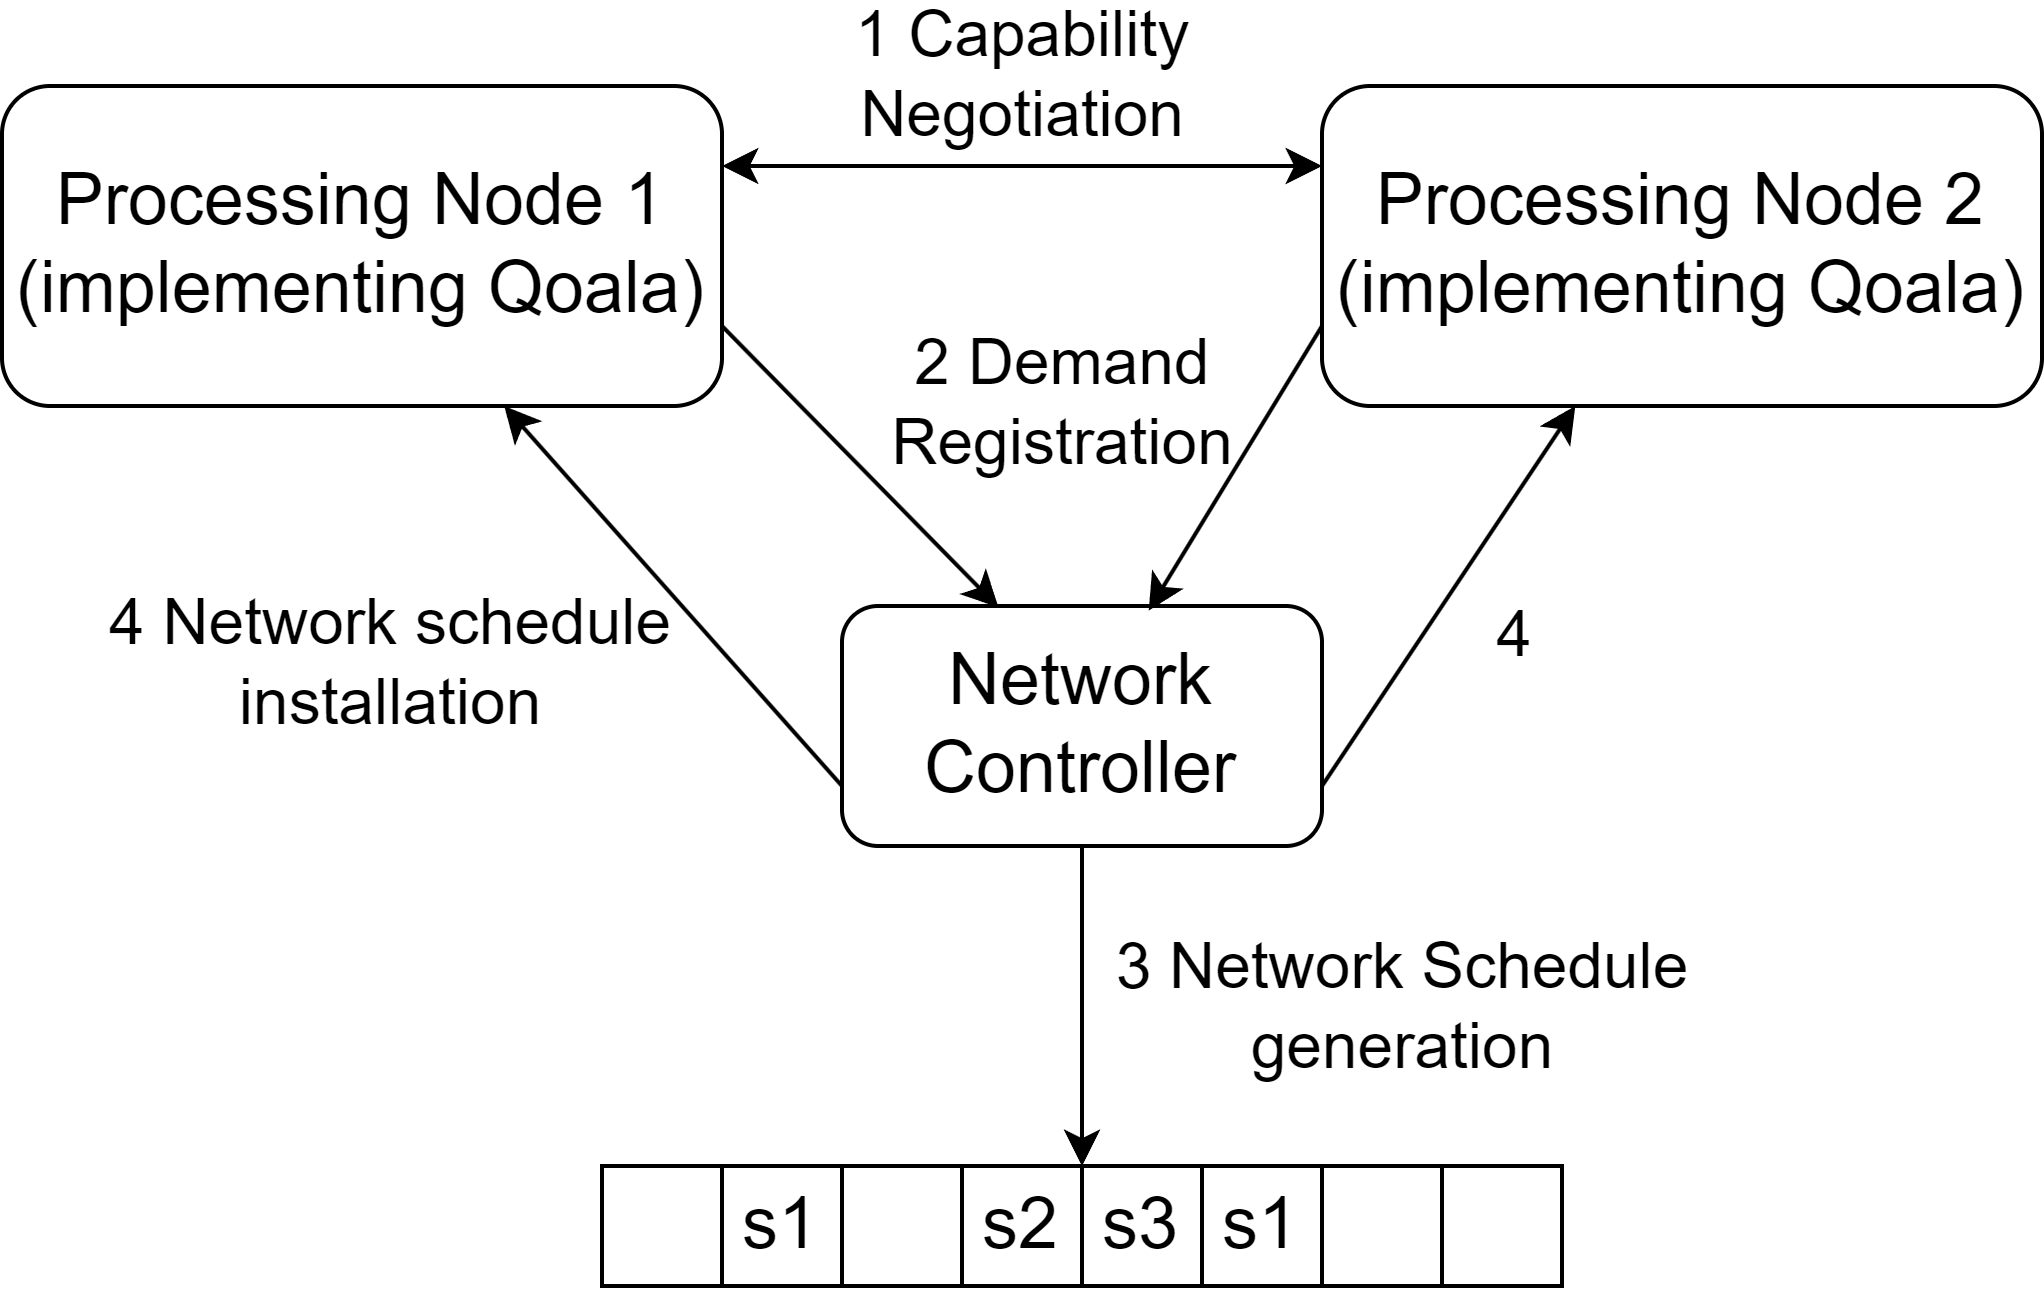
\includegraphics[scale=0.8]{figures/qoala/network_controller_setup.png}
    \caption{High-level steps of using the network controller.
    1. Nodes discuss among each other constraints about application execution (Capability Negotiation).
    2. The outcome of Capability Negotiation, which contains demands about entanglement generation, is sent to the network controller (Demand Registration).
    3. Based on the demands from the nodes, the network controller constructs a network schedule consisting of time slots. Each time slot is assigned to zero or more \textit{sessions}, which correspond to program instance pairs.
    }
    \label{fig:app:network_controller_setup}
\end{figure*}

\textbf{On-demand entanglement requests.} At runtime, nodes implementing Qoala may send requests to the \textit{network stack}.
This network stack then issues \textit{EPR requests} to the network controller.
Upon receiving an EPR request, the network controller stores it and potentially acts on it:
\begin{itemize}
    \item If there is a matching EPR request from the other node, and if the current time slot is assigned to the corresponding session, perform the actual entanglement generation process.
    \item If at least one of the two above conditions does not hold, keep the request until both conditions are satisfied (a matching request from the other node arrives, or the corresponding time slot arrives, or both).
\end{itemize}

An EPR request is a request for a single EPR pair. A \texttt{SinglePair} task is handled by the network stack sending a single EPR request to the network controller.
A \texttt{MultiPair} task is handled by sending multiple EPR requests, possibly interleaved by local QPS processing such as callback routines.

The network stack may fail handling a request. For example, it might timeout trying to produce an EPR pair. In this case, the corresponding task (\texttt{SinglePair} or \texttt{MultiPair}) also fails.
Depending on the scheduler implementation, this task may be executed again at a later time, or the whole program instance may be aborted.


\textbf{Entanglement generation as a black box.} We assume that all nodes can create entanglement with all nodes, orchestrated by the network controller.
Qoala does not assume anything about the existence of repeater nodes or entanglement routing algorithms.
Rather, a node sending a request for entanglement (in a suitable time slot) will either get this entanglement (created in some way, irrelevant to Qoala) or not (creation failed for some reason, again irrelevant to Qoala).
The network stack and controller may be implemented in various ways, such as illustrated in Figure~\ref{fig:app:network_controller_types}.


\subsection{Detailed runtime overview}
Figure~\ref{fig:app:runtime_detailed} provides an overview of the runtime architecture.